\section{HOPG-Probe}\label{sec:hopg-probe}
\subsection*{Struktur}
Hochorientierter pyrolytischer Graphit (HOPG) ist kristalliner Kohlenstoff, wo Atome einer Schicht
auf einem hexagonalen Gitter geordnet sind, wodurch jedes Atom auf dieser zweidimensionalen
Ebene von drei weiteren Atomen im Winkel von \SI{120}{\degree} verbunden ist. Zwei Schichten
dieses Gitters sind versetzt übereinander geordnet (siehe \cref{fig:hopg-skizze}), weshalb durch die
untere Ebene die Ladungsverteilung auf der Oberfläche beeinflusst wird.\par Wie in
\cref{fig:hopg2} erkennbar, ist bei den H-Atomen die Ladungsverteilung minimal und bei A-Atomen maximal.
Die Verteilung bei den B-Atomen befindet sich dazwischen, weshalb diese für das Mikroskop unsichtbar werden,
da ein RTM nicht unmittelbar die Oberflächentopographie messen kann, sondern die Aufenthaltswahrscheinlichkeit der
Elektronen \cite{rtm-leitpfaden}.

%bilder von HOPG Struktur
\begin{figure}[htb]
	\centering
	\begin{subfigure}{0.45\linewidth}
		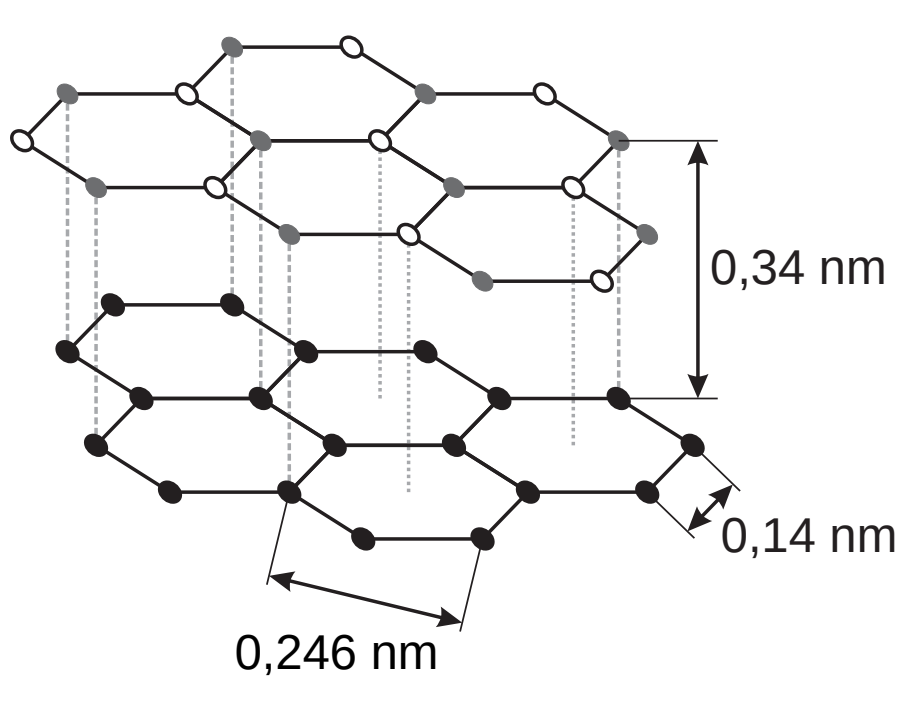
\includegraphics[width=\linewidth]{figs/hopg1.png}
		\caption{Seitenansicht.\cite{skript}}
		\label{fig:hopg1}
	\end{subfigure}
	\hspace{0.5cm}
	\begin{subfigure}{0.45\linewidth}
		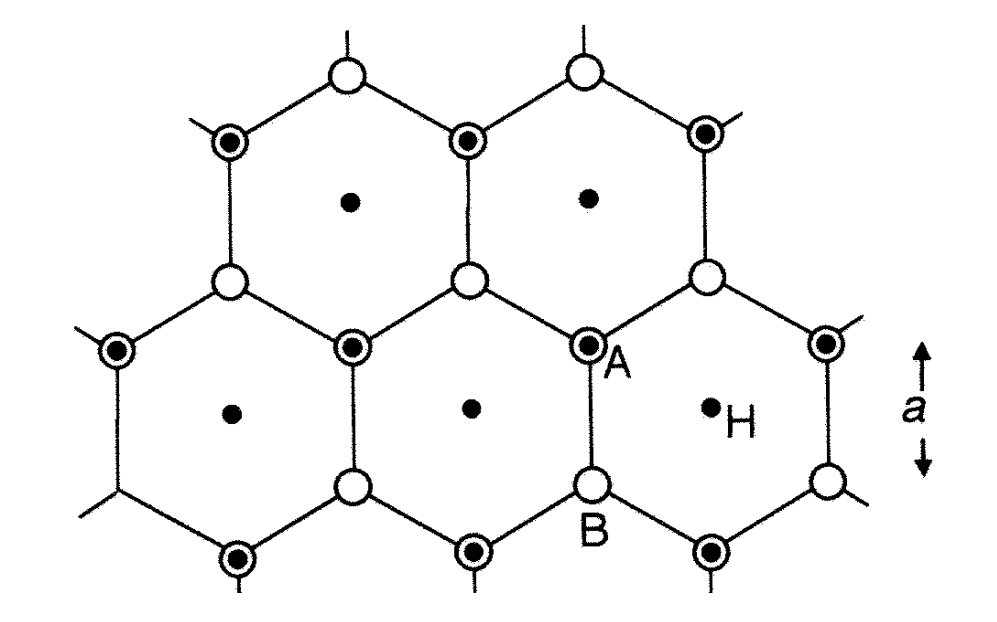
\includegraphics[width=\linewidth]{figs/hopg2.png}
		\caption{Obere Ansicht.\cite{rtm-leitpfaden}}
		\label{fig:hopg2}
	\end{subfigure}
	\caption{Hochorientierter pyrolytischer Graphit.}
	\label{fig:hopg-skizze}
\end{figure}

\subsection*{Vorbereitung}
Im Gegensatz zu Gold wird hier versucht, die atomare Struktur des Graphits aufzulösen.
Dies erfordert hohe Präzision in der Durchführung und der Präparierung der Spitze. Der Platin-Iridium-Draht
vor der Rasterung ist in \cref{fig:spitze_hopg_vorher_v2} abgebildet. Vorne ist eine dünne Spitze zur ekennen,
die sich für die Durchführung eignen sollte.

\begin{figure}[htb]
	\centering
	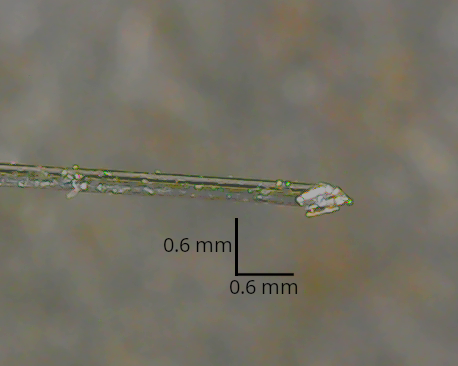
\includegraphics[width=0.5\linewidth]{figs/spitze_hopg_vorher_v2.png}
	\caption{Platin-Iridium-Spitze (Spitze 2) vor Rasterung des HOPG.}
	\label{fig:spitze_hopg_vorher_v2}
\end{figure}

Die Graphit-Probe ist in \cref{fig:usb_mikroskop_hopg} mit zwei unterschiedlichen
Vergrößerungen abgebildet. Zu erkennen ist eine Stufenstruktur auf der Oberfläche, die jedoch
deutlich größer ist als die Fläche, die gerastert werden soll. Daher kann mit dieser
Probe gearbeitet werden.

% USB-Mikroskop Bilder von HOPG
\begin{figure}[htb]
	\centering
	\begin{subfigure}{0.45\linewidth}
		\centering
		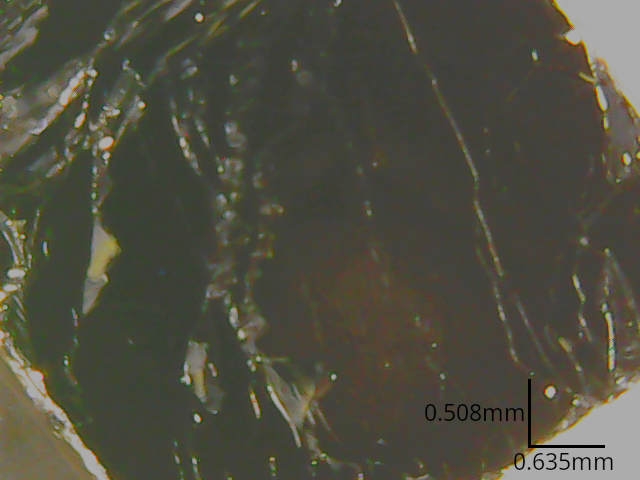
\includegraphics[width=\linewidth]{figs/hopg_skala1.png}
		\caption{Skala 1}
		\label{fig:hopg_skala1}
	\end{subfigure}
	\hspace{0.5cm}
	\begin{subfigure}{0.45\linewidth}
		\centering
		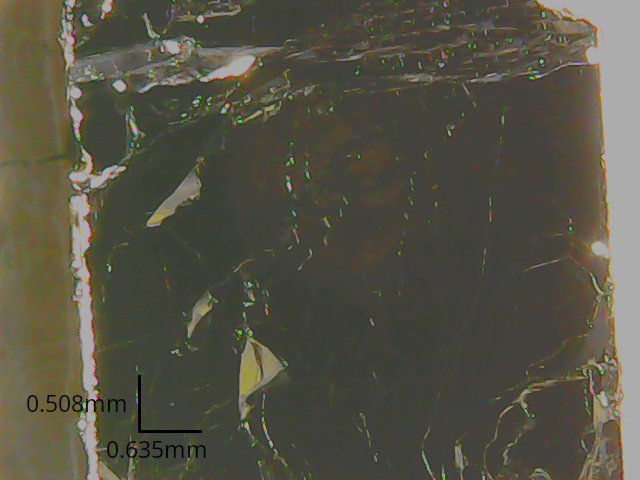
\includegraphics[width=\linewidth]{figs/hopg_skala2.png}
		\caption{Skala 2}
		\label{fig:hopg_skala2}
	\end{subfigure}
	\caption{USB-Mikroskop Aufnahmen von HOPG nach Abziehen der obersten Schicht.}
	\label{fig:usb_mikroskop_hopg}
\end{figure}

\subsection*{Auswertung}

Nach erfolgreicher Annäherung der Probe an die Spitze wird zunächst ein Bild
mit einer großen Breite gemacht, um die Grobstruktur der Oberfläche
zu bekommen um damit einen ausreichend flachen Flächenabschnitt
finden zu können. Die Abbildungen und die Längenabmessungen der Messdaten wurden 
mit der Software \verb|Gwyddion| erstellt. Ein Bild bei einer Breite von $\SI{200}{\nm}$ ist in
\cref{fig:hopg_rtm_weitaufnahme} zu sehen, wobei das obere rechte Viertel
von einer flachen Ebene gefüllt wird, wo hier die Höhenschwankung maximal \SI{1}{\nm} beträgt.

\begin{figure}[htb]
	\centering
	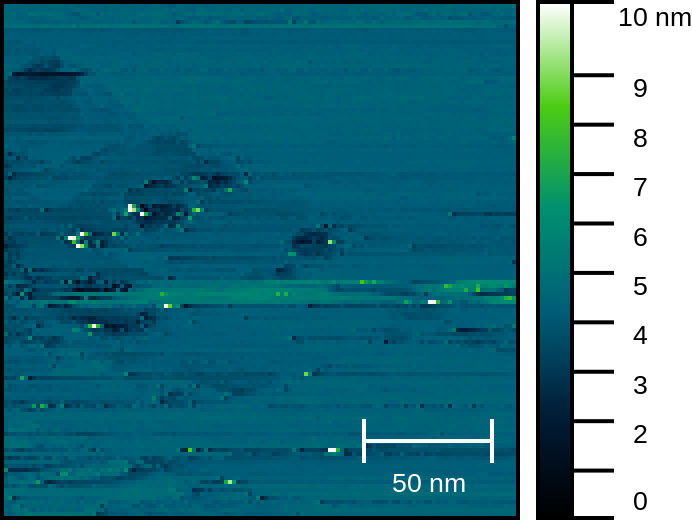
\includegraphics[width=0.6\linewidth]{figs/HOPG10558.png}
	\caption{RTM-Aufnahmen der HOPG-Probe. \textit{Image size} \SI{200}{\nano \meter},
		\textit{Rastergeschwindigkeit} \SI{1}{\micro\m\per \second}, \textit{Setpoint} \SI{5}{\nano \ampere},
		\textit{Tip voltage} \SI{0.5}{\volt}, \textit{P-Gain} \num{1000}, \textit{I-Gain} \num{2000},
		\textit{D-Gain} \num{0}, Spitze 2.}
	\label{fig:hopg_rtm_weitaufnahme}
\end{figure}

Nach Auswahl eines kleineren Gebiets konnten RTM-Aufnahmen in einer Größenordnung gemacht werden, wo 
Atomstrukturen sichtbar werden sollen. Diese Aufnahmen sind in \cref{fig:hopg_rtm_1,fig:hopg_rtm_2} zu sehen, wobei 
die linke Aufnahme die Strommessung und die rechte Aufnahme die Abstandsmessung auf dem Hinweg darstellt.
Die Abstände wurden dabei auf das Minimum der Messung normiert.\par
Die Abstandsmessung zeigt, dass die 
Spitze auf einer horizontalen Linie stets die selbe Höhe aufweist und lediglich auf der vertikalen leicht variiert ist.
Diese Variation liegt in Aufnahme \ref{fig:hopg_rtm_1} unter \SI{57}{\pm} und in Aufnahme \ref{fig:hopg_rtm_1}
unter \SI{40}{\pm}. Diese Schwankungen sind kleiner als ein Atomdurchmesser und könnten durch eine noch 
vorhandene leichte Neigung der Spitzen-Ebene in Relation zur Proben-Oberfläche entstanden sein, möglich sind auch 
thermische Ausdehnung oder Störungen durch Vibrationen. Da wie zu sehen diese Schwankungen klein sind, kann 
trotzdessen eine konstante Höhenmessung angenommen werden, womit die Strommessung unmittelbar die 
Ladungsverteilung der Oberläche darstellt.

\begin{figure}
	\centering
	\begin{subfigure}{0.45\linewidth}
		\centering
		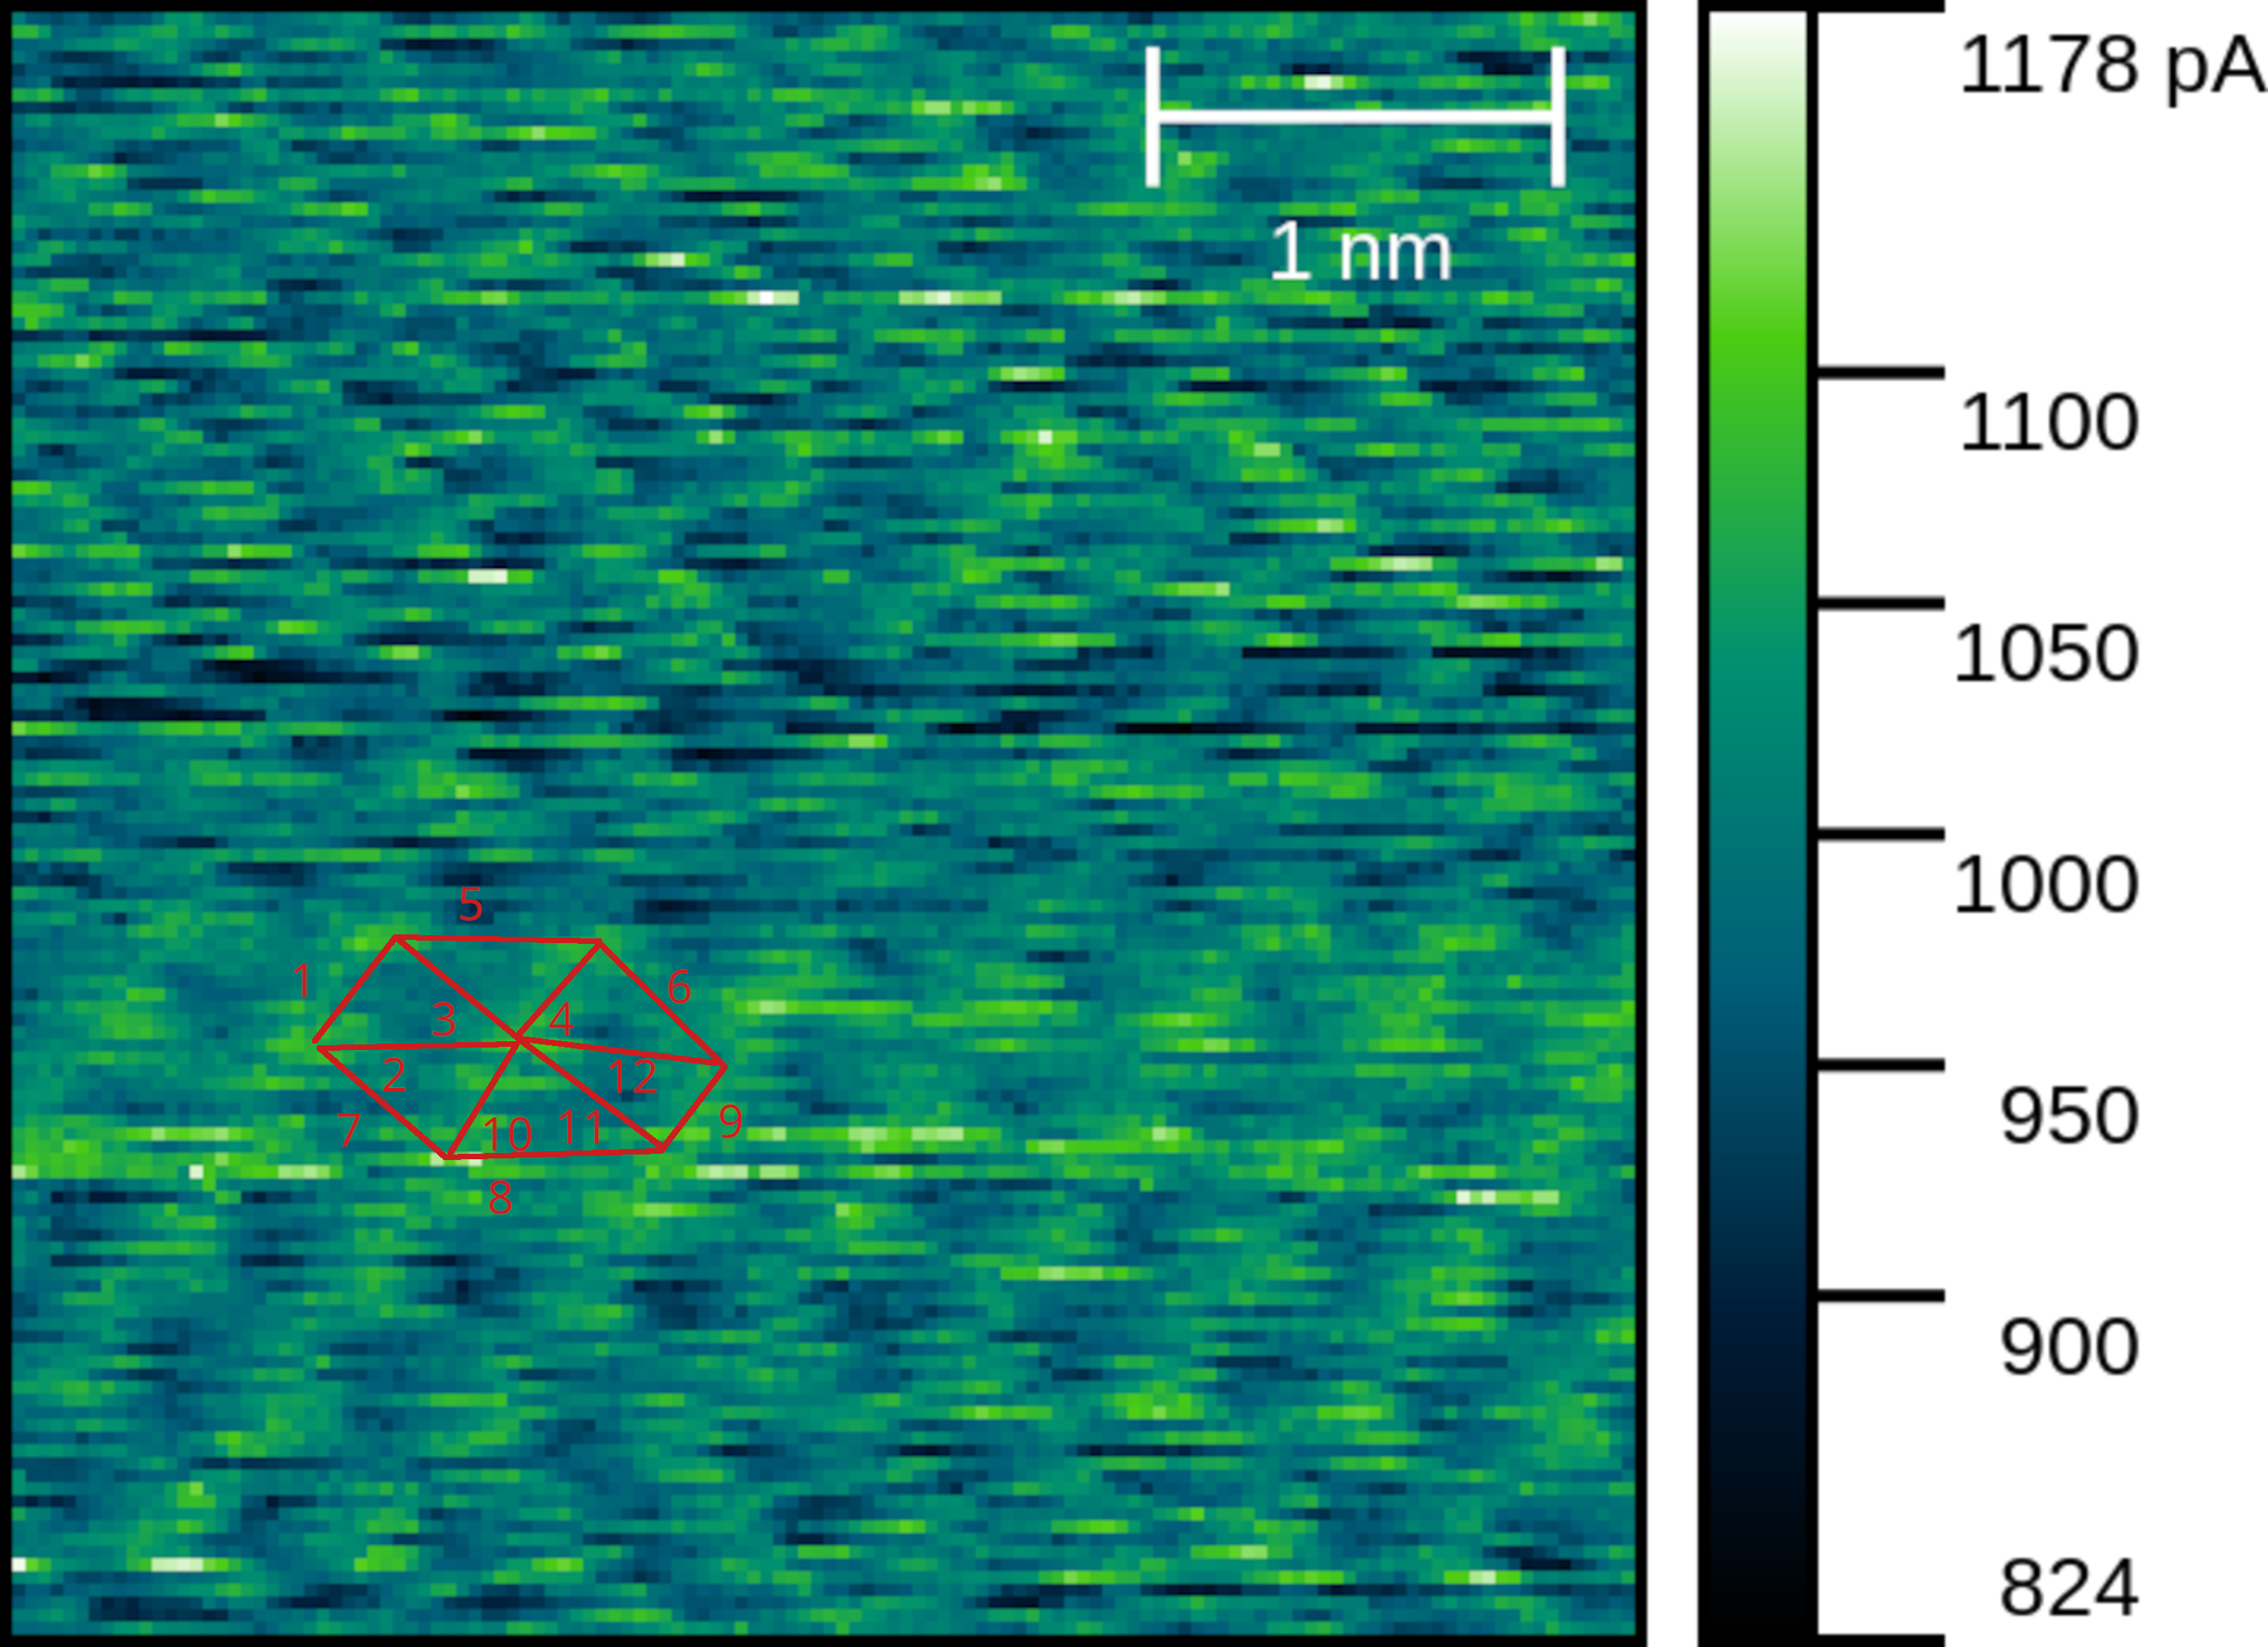
\includegraphics[width=\linewidth]{figs/HOPG10597_lines.png}
		\caption{Strommessung}
		\label{fig:hopg_rtm_4nm_1_cur}
	\end{subfigure}
	\hspace{.5cm}
	\begin{subfigure}{0.45\linewidth}
		\centering
		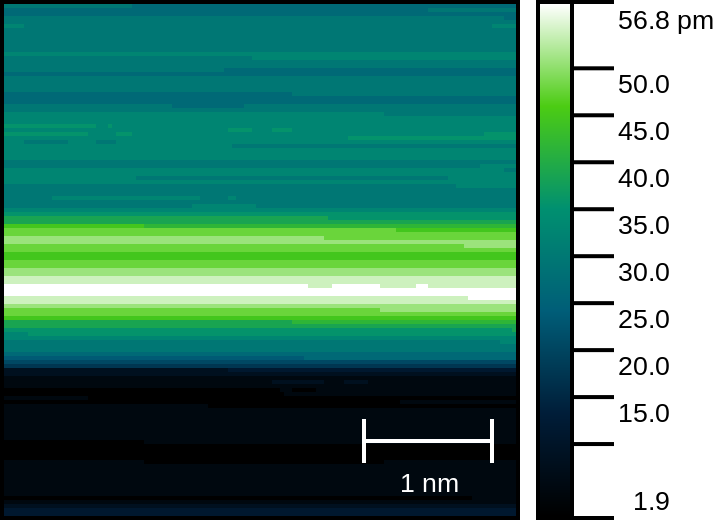
\includegraphics[width=\linewidth]{figs/HOPG10597_height.png}
		\caption{Abstandsmessung}
		\label{fig:hopg_rtm_4nm_1_height}
	\end{subfigure}
	\caption{RTM-Aufnahmen der HOPG-Probe. \textit{Image size} \SI{4}{\nano \meter},
	\textit{Rastergeschwindigkeit} \SI{77.5}{\nm\per \second}, \textit{Setpoint} \SI{1}{\nano \ampere},
	\textit{Tip voltage} \SI{0.1}{\volt}, \textit{P-Gain} \num{0}, \textit{I-Gain} \num{4},
	\textit{D-Gain} \num{0}, Spitze 2, \textit{Rotation} \SI{20}{\degree}.}
	\label{fig:hopg_rtm_1}
\end{figure}

\begin{figure}
	\centering
	\begin{subfigure}{0.45\linewidth}
		\centering
		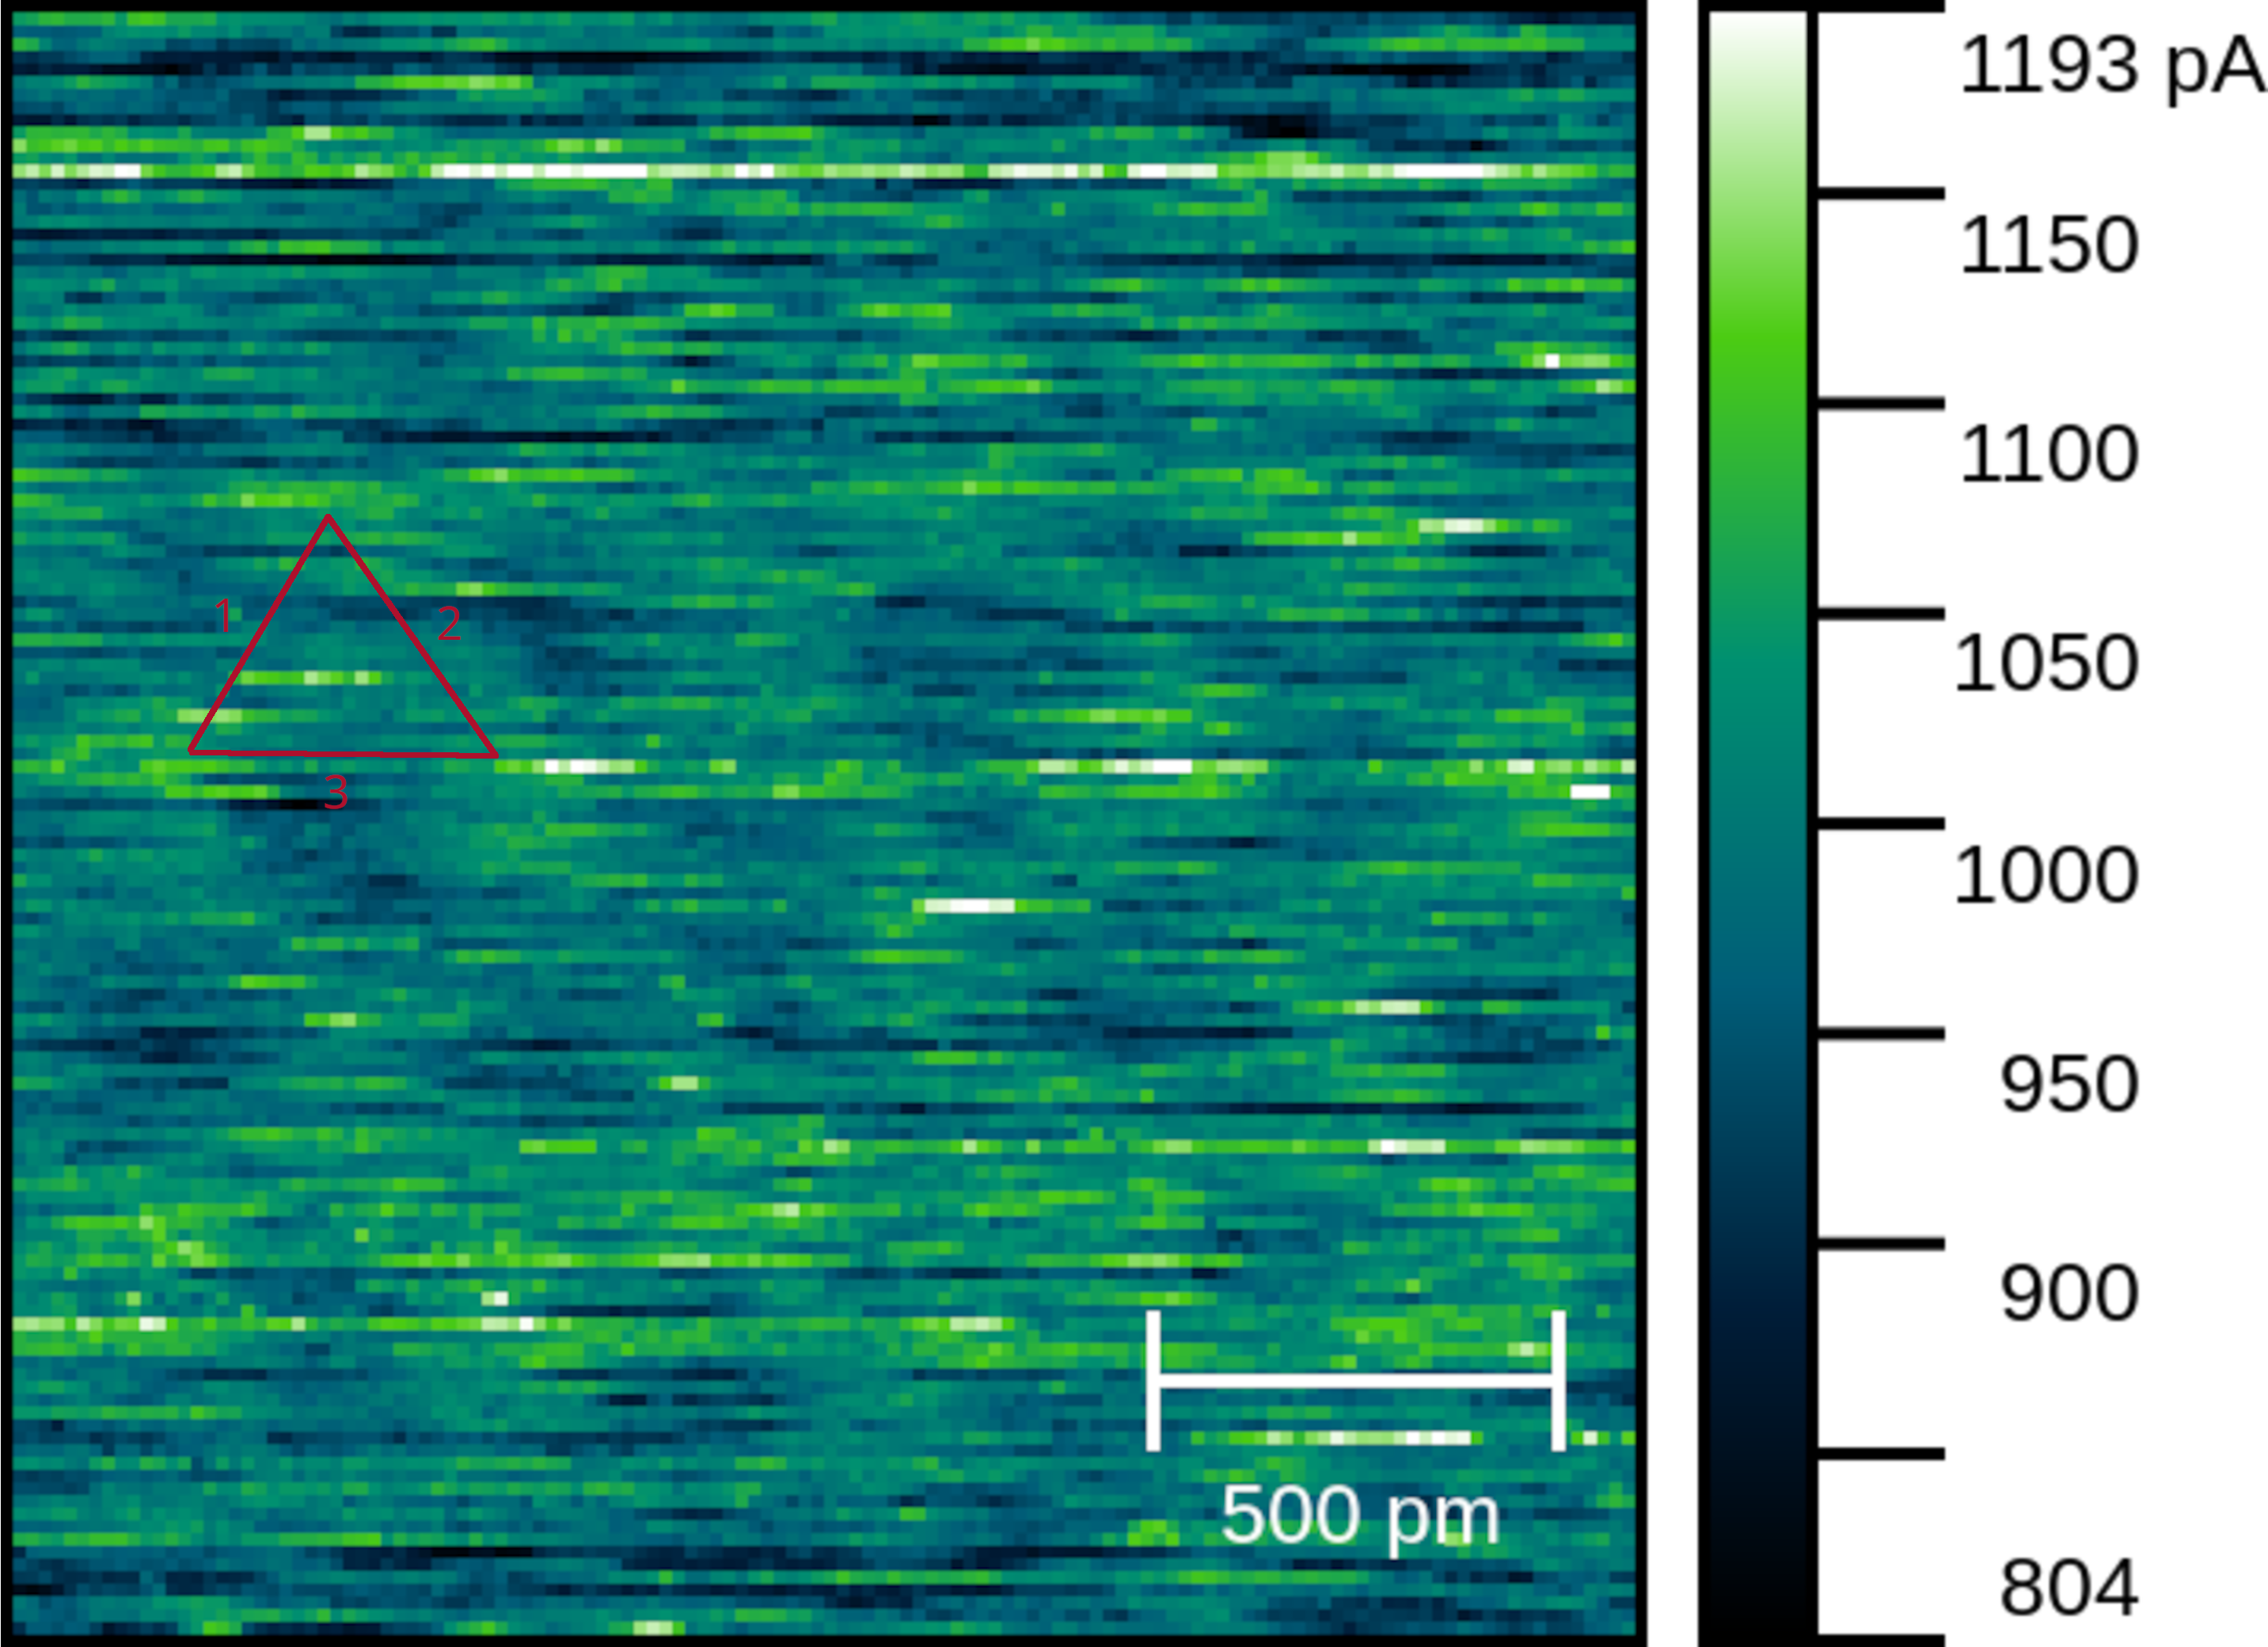
\includegraphics[width=\linewidth]{figs/HOPG10628_lines.png}
		\caption{Strommessung}
		\label{fig:hopg_rtm_4nm_2_cur}
	\end{subfigure}
	\hspace{.5cm}
	\begin{subfigure}{0.45\linewidth}
		\centering
		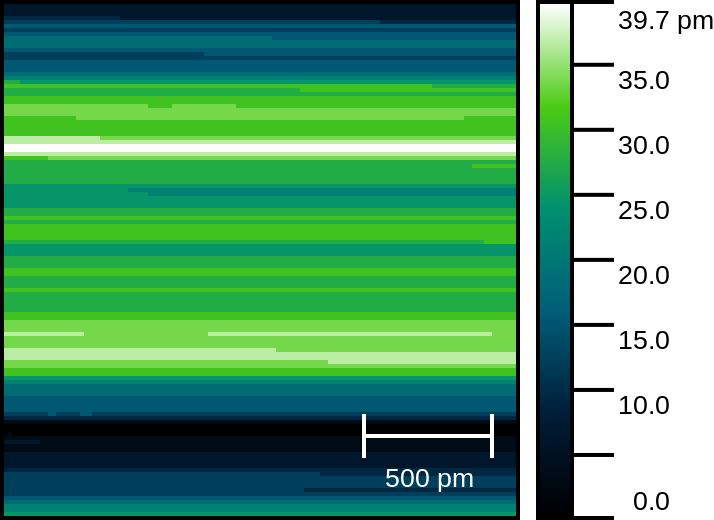
\includegraphics[width=\linewidth]{figs/HOPG10628_height.png}
		\caption{Abstandsmessung}
		\label{fig:hopg_rtm_4nm_2_height}
	\end{subfigure}
	\caption{RTM-Aufnahmen der HOPG-Probe. \textit{Image size} \SI{2}{\nano \meter},
	\textit{Rastergeschwindigkeit} \SI{77.5}{\nm\per \second}, \textit{Setpoint} \SI{1}{\nano \ampere},
	\textit{Tip voltage} \SI{0.1}{\volt}, \textit{P-Gain} \num{0}, \textit{I-Gain} \num{4},
	\textit{D-Gain} \num{0}, \textit{Rotation} \SI{20}{\degree}}
	\label{fig:hopg_rtm_2}
\end{figure}

In \cref{fig:hopg_rtm_4nm_1_cur} ist in der unteren Hälfte deutlich nach \cref{fig:hopg2} die erwartete Struktur 
von HOPG zu erkennen, jedoch mit einer geringen Auflösung. Diese konnte nach Variation der 
RTM-Parameter nicht verbessert werden. Der Grund hierfür ist mit höchster Wahrscheinlichkeit die Topographie 
der Spitze, da die Höhe dieser konstant gehalten wurde und ebenso ausreichend nah an die Probe 
herangefahren wurde, sodass Ströme von bis zu \SI{1}{\nano\ampere} gemessen wurden.\par
Trotzdessen ist die Auflösung hoch genug, um quantitativ die Atomabstände abschätzen zu können.
In \cref{fig:hopg_rtm_4nm_1_cur} sind in rot Linien eingezeichnet, die die Abstände der A-Atome (siehe 
\cref{fig:hopg2}) zeigen. Dies wurde für sieben aneinander liegenden Atomen gemacht. Auffällig ist
hierbei, dass die erwartete Symmetrie der Abstände zueinander nicht vorhanden ist, da in 
x-Richtung die gemessenen Längen größer sind als in y-Richtung. Im Falle, dass das Mikroskop 
die Linien vertikal abrastert, kann diese Streckung der Abstände durch thermische Ausdehnung 
erklärt werden, weswegen sich während des Versuchs die Probe leicht in ihrer Position verschoben
hätte. Eine weitere Option sei hierbei kein Messfehler, sondern eine 
fehlerhafte Eichung des Piezos, da HOPG aufgrund seiner Struktur in der Praxis zur 
Eichung genutzt wird. Die Messwerte sind in \cref{tab:atomabstand} mit $\varphi_1$ für den Winkel der 
Linie relativ zur horizontalen Achse der Aufnahme und $r_1$ für die Länge denotiert. Die 
Fehler wurden für den Winkel mit \SI{10}{\degree} und die Länge mit \SI{90}{\pm} aufgrund 
der Auflösung gewählt.\par


Die Linien formen ein Sechseck bestehend aus sechs einzelnen Dreiecken, die nach Grahpit-Struktur alle 
gleichseitig zu erwarten sind. Dies ist jedoch hier nicht der Fall. Es ist zu erkennen, dass Längen 
in y-Richtung sich in einem Bereich von \SI{290}{\nm} befinden, während Längen mit höheren Anteil 
in x-Richtung größer als \SI{400}{\pm} sind. Die Streckung in x-Richtung wird durch zu kleine Winkel 
der Linien 3, 6 und 7 deutlich.\par 
Der Mittelwert der Abstände liegt hier bei 
\begin{equation}
	d_1 = \SI{380\pm 160}{\pm}, 
	\label{abstand_rtm_1}
\end{equation}
wobei sich der Fehler aus der Standardabweichung der Messung sowie den einzelnen Fehlern zusammensetzt. 
Mit einem hohen Fehler von \SI{42}{\percent} liegt der in \cite{skript} angegebene Literaturwert von 
\SI{246}{\nm}
im $1\sigma$-Bereich der Messung, wobei die Messung eine Abweichung nach oben hin darstellt.\\\par 

In Aufnahme \ref{fig:hopg_rtm_4nm_2_cur} konnte aufgrund von schlechter Auflösung 
nur für drei Linien am linken Rand der Abbildung der Atomabstand ausgewertet werden. Die Fehler für 
die Winkel $\varphi_2$ sind wieder mit \SI{10}{\degree} bestimmt worden und der 
Fehler der Abstände $r_2$ mit \SI{100}{\pm}. Hier kann ein mittlerer Abstand von 
\begin{equation}
	d_2 = \SI{390\pm140}{\pm}
	\label{abstand_rtm_2}
\end{equation}
bestimmt werden, was sich mit dem Messwert \ref{abstand_rtm_1} überlagert.

\begin{table}[htbp]
   \centering
\caption{relative Winkel zur Horizontalen und eingezeichnete Abstände aus \cref{fig:hopg_rtm_4nm_1_cur,fig:hopg_rtm_4nm_2_cur}}
\begin{tabular}{c c c c c}
\hline Linie & $\varphi_1 / {}^\circ$ & $r_1/\unit{\pm} \pm \SI{90}{\pm}$ & $\varphi_2 / {}^\circ$ & $r_2/\unit{\pm} \pm \SI{100}{\pm}$ \\ 
\hline
$\num{1}$ & $\num{52.0}$ & $\num{340}$ & $\num{50.1}$ & $\num{300}$ \\
$\num{2}$ & $\num{-3.1}$ & $\num{490}$ & $\num{-53.1}$ & $\num{400}$ \\
$\num{3}$ & $\num{-41.8}$ & $\num{410}$ & $\num{-6.0}$ & $\num{400}$ \\
$\num{4}$ & $\num{58.1}$ & $\num{290}$ &    &    \\
$\num{5}$ & $\num{-7.4}$ & $\num{460}$ &    &    \\
$\num{6}$ & $\num{-45.0}$ & $\num{420}$ &    &    \\
$\num{7}$ & $\num{-40.2}$ & $\num{390}$ &    &    \\
$\num{8}$ & $\num{-4.1}$ & $\num{460}$ &    &    \\
$\num{9}$ & $\num{52.4}$ & $\num{290}$ &    &    \\
$\num{10}$ & $\num{58.1}$ & $\num{290}$ &    &    \\
$\num{11}$ & $\num{-48.0}$ & $\num{350}$ &    &    \\
$\num{12}$ & $\num{-6.1}$ & $\num{430}$ &    &    \\
\hline\end{tabular}
\end{table}

Die Rasterspitze nach der Messung ist in \cref{fig:spitze_hopg_nachher} gezeigt. Zu sehen ist 
wie vorher eine sehr dünne Spitze, die nach visueller Bewertung eine höhere Auflösung hätte erreichen sollen.

\begin{figure}[htb]
	\centering
	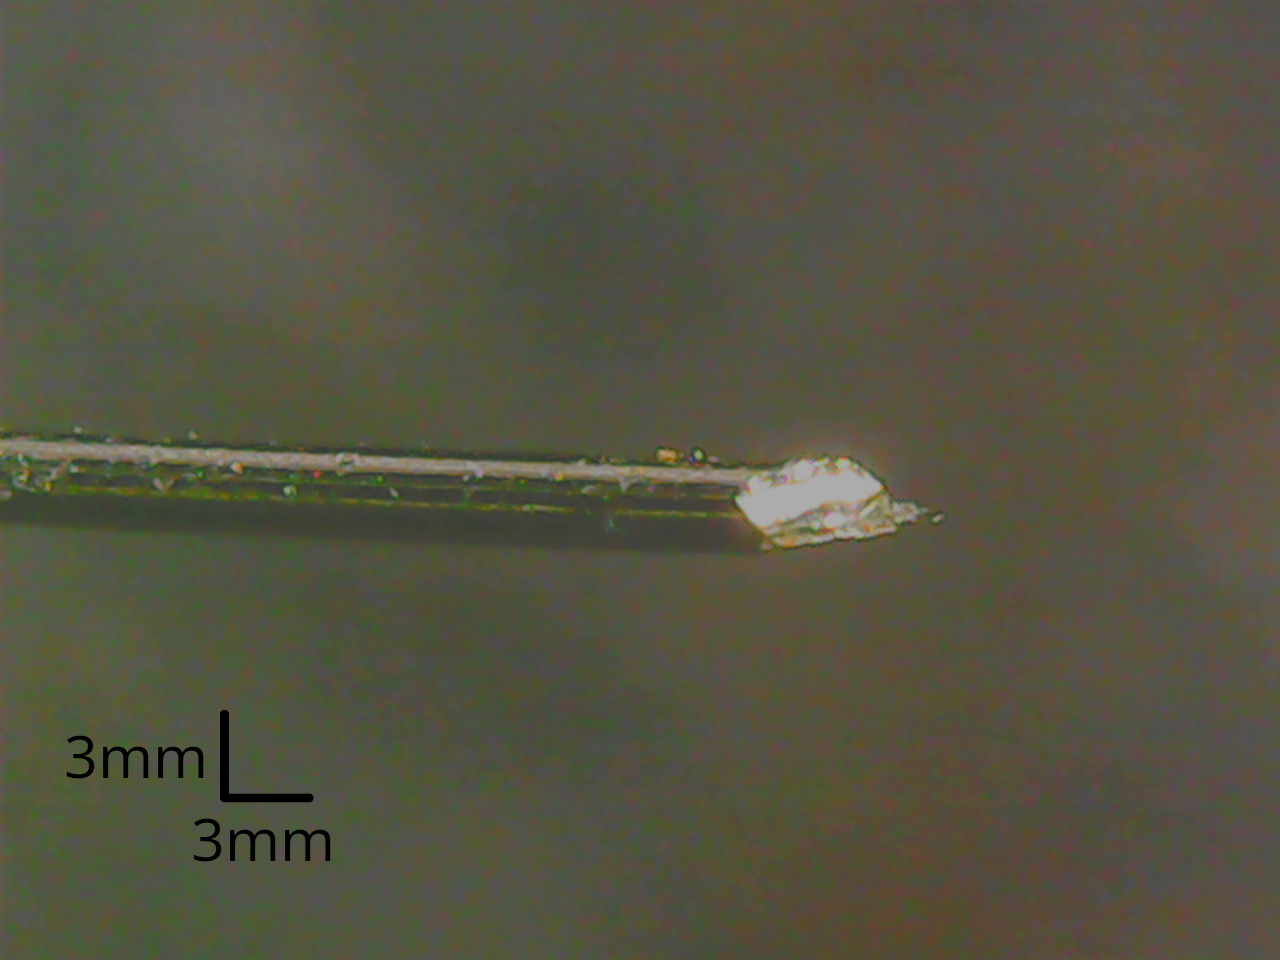
\includegraphics[width=0.5\linewidth]{figs/spitze_hopg_nachher_v2}
	\caption{Platin-Iridium Spitze nach Rasterung des HOPG.}
	\label{fig:spitze_hopg_nachher}
\end{figure}
